\chapter{Background}

\section{ASP.NET Web Forms} % (fold)
\label{sec:asp_net_web_forms}
	% Todo: explain Active Server Pages
	ASP.NET Web Forms are the User Interface (UI) elements that give your web applications their look and feel. Web Forms are similar to Windows Forms \cite{msdn01} in that they provide properties, methods, and events for the controls that are placed onto them. However, these UI elements render themselves into Html \cite{msdn02}. When working with Web Forms you can both write markup code and write C\# code when building a web page. 

	\begin{figure}[H]
					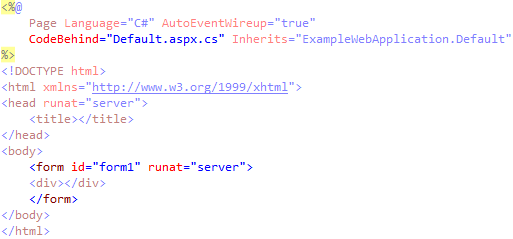
\includegraphics[width=12cm]{resources/images/Markup.png}
				\caption{Markup code for the empty page \texttt{Default.aspx}}
				\label{markup}
			\end{figure}

	\subsection{Code Behind} % (fold)
	\label{sub:code_behind}
		The web page \texttt{Default.aspx} is associated to the C\# file \texttt{Default.aspx.cs}. This is the \texttt{Default.aspx} page's \emph{Code Behind} file. 

		Web pages in ASP.NET Web Forms have different server side events that can be accessed from Code Behind. In figure \ref{codeBehind} the page load event is used to a button control to the form \texttt{form1} (\texttt{form1} was defined in the markup in figure \ref{markup}). This is how HTML elements are added from Code Behind which is opposed to adding them in markup code.


				\begin{figure}[H]
					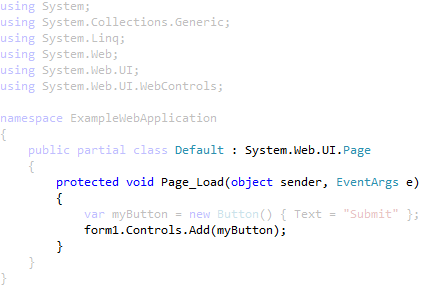
\includegraphics[width=10cm]{resources/images/CodeBehind.png}
				\caption{\texttt{Default.aspx.cs} Code Behind file of the page \texttt{Default.aspx}.}
				\label{codeBehind}
			\end{figure}
		
		A page's server side events are triggered on every request to the page's URL. In this case the resulting web page and source is as shown in figure \ref{html}.

				\begin{figure}[H]
					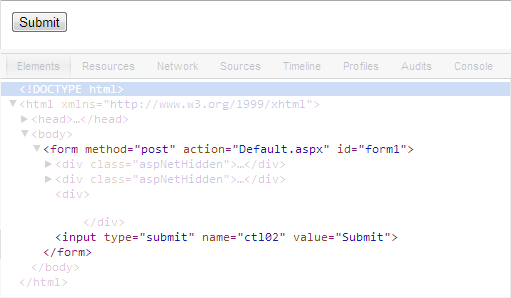
\includegraphics[width=12cm]{resources/images/Html.png}
				\caption{Resulting web page and source code of the Default.aspx page (shown with Chrome Development Tools).}
				\label{html}
			\end{figure}

		In ASP.NET Web Forms there are built-in control classes equivalent to most HTML elements, so in this manner one can build an entire web application from Code Behind.

		\subsection{Client Side Scripts \& Code Behind} % (fold)
		\label{sub:client_side_scripts_code_behind}
			When working from Code Behind client side scripts can e.g. be added to a button's client side click event by setting the button's \texttt{OnClientClick} property (see Figure \ref{buttonScript}). Another approach would be to register a script with the \texttt{ScriptManager} object that should be associated to the specific page.

		\begin{figure}[H]
			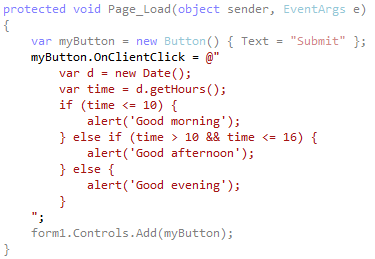
\includegraphics[width=9cm]{resources/images/ButtonScript.png}
			\caption{Script registered with button's client side click event.}
			\label{buttonScript}
		\end{figure}

		Common for both approaches is that JavaScript is added as text strings which can be considered somewhat unsafe.
		% subsubsection subsubsection_name (end)

	% subsection code_behind (end)

% section asp_net_web_forms (end)

\section{JavaScript and its Unsafe Language Features} % (fold)
\label{sec:javascript_and_its_unsafe_language_feature}
	
	JavaScript is an interpreted, dynamically typed scripting language used mainly for making web applications with dynamic user interfaces. JavaScript inherits its syntax from C, and was developed by Netscape in 1995 \cite{bib:wiki_javascript}. Today, JavaScript is used in almost all big web applications, but despite its popularity, it has some language features that can be considered unsafe. The remainder of this section will highlight some of these unsafe language features.

	\subsection{No Comepile Time Validation} % (fold)
	\label{sub:no_compile_time_validation}
		In general enforcing correctness at compile time instead of runtime makes the development process safer as some errors (e.g.\ syntax errors like missing semicolons) are not possible to overlook or ignore. Furthermore discovering errors as early as possible makes the debugging process easier hence compile time errors should be preferred over runtime errors. So the fact that JavaScript is an interpreted language that is not compiled makes it a less safe language.
	% subsection no_compile_time_validation (end)

	\subsection{Dynamic Type System} % (fold)
	\label{sub:dynamic_type_system}
		JavaScript has a dynamic type system which in some situations makes the development process faster but also less safe as some errors will not emerge at all (or maybe emerge at runtime). E.g. it is possible to add a \texttt{Number} value with a \texttt{Boolean} value without getting any warnings. In other words it is possible to forget enforcing that a variable has a specific type. This problem is amplified when parsing external input as it is done e.g.\ in form validation.
	% subsection dynamic_type_system (end)

	\subsection{Reuse of Identifiers in Declarations} % (fold)
	\label{sec:reuse_of_identifiers_in_declarations}
		JavaScript allows declaring multiple variables or functions with the same name in the same execution context without any warnings. This makes it possible by mistake to override earlier declared variables or functions. This kind of errors can be difficult and time consuming to discover because of their hidden nature.
	% section reuse_of_identifiers_in_declarations (end)

	\subsection{No Block Scope} % (fold)
	\label{sub:no_block_scope}
		JavaScript's syntax comes from C. In all other C-like languages a block creates scope. This is not the case in JavaScript even though its block syntax suggests that it does (Crockford (2008) p. 102 \cite{good_parts}). This can be a source of confusion especially for programmers that are used to block scope. Scope related errors might be difficult to debug as obviously no warnings are given (since there is no block scope) when a variable from an outer block is assigned a value by mistake.
	% subsection no_block_scope (end)

	\subsection{Implicit Type Conversion} % (fold)
	\label{sub:implicit_type_conversion}
	TODO
	% subsection implicit_type_conversion (end)

	\subsection{Many ''Falsy'' Values} % (fold)
	\label{sub:many_falsy_values}
		JavaScript has multiple falsy values which are seen in Figure \ref{falsyValues}.

			\begin{figure}[H]
				\begin{center}
					\centerline{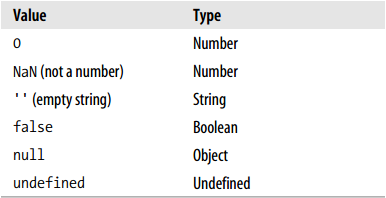
\includegraphics[width=9cm]{resources/images/FalsyValues.png}}
				\end{center}
				\caption{Table of JavaScript ''falsy'' values \cite{good_parts}}
				\label{falsyValues}
			\end{figure}

		These values are all ''falsy'', but they are not interchangeable. For example, Figure \ref{falsyExample} shows the wrong way to determine if an object is missing a member (Crockford (2008) p. 106 \cite{good_parts}).

					\begin{figure}[H]
				\begin{center}
					\centerline{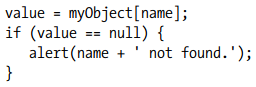
\includegraphics[width=6cm]{resources/images/FalsyExample.png}}
				\end{center}
				\caption{Incorrect way of using the ''falsy'' value \texttt{null} \cite{good_parts}}
				\label{falsyExample}
			\end{figure}

		Multiple ''falsy'' values is another source of errors that can be difficult to discover.
	% subsection many_falsy_values (end)
% section javascript_and_its_unsafe_language_feature (end)

\section{Related works} % (fold)
\label{sec:related_works}
	There are many existing projects that makes writing JavaScript in safe manner possible. To name a few one could mention Microsoft’s TypeScript, Google Web Toolkit (GWT) or Script\#. There is however many different approaches to writing JavaScript safely. TypeScript is a superset of JavaScript i.e.\ it extends the JavaScript language with safe language features like static typing. GWT is a cross compiler from Java to JavaScript. Script\# is also a cross compiler but from C\# to JavaScript.
% section related_works (end)

